In order to verify and validate the design, each module is tested and compared with simulation results. The corresponding tests verify the feasibility of the design.

Measurements of the clock generator and one phase of the RF field (RF+) are shown in the Fig. \ref{fig:meas}.a. The waveform demonstrates that the CG works as expected and in fact divides the clock frequency (13.56MHz/4). The clock signal ripple is due to the noise of the external power source to which the ring pad is connected. 

Fig. \ref{fig:meas}.b shows the comparison between RF+ with the output of the POR module, where the delay of the POR in relation to the input signal. This delay allows the DPU to enter into idle state.

Finally, Fig. \ref{fig:meas}.c shows the signal recovery transmitted from the PCD. It demonstrates that the clock is interrupted whenever a frame arrives.

\begin{figure}[h]
  \centering
  \includegraphics[page=20,width=80mm]{images-crop.pdf}
  \caption{(a) Clk/4 vs RF+, (b) RF+ vs POR, (c) Clk/4 vs Demodulator}
  \label{fig:meas}
\end{figure}